\section{Eigenschaften von Funktionsgraphen}
\subsection{Achsenschnittpunkte und Monotonie}
\begin{LA}
    {Einführungsaufgabe}{}
    \begin{center}
        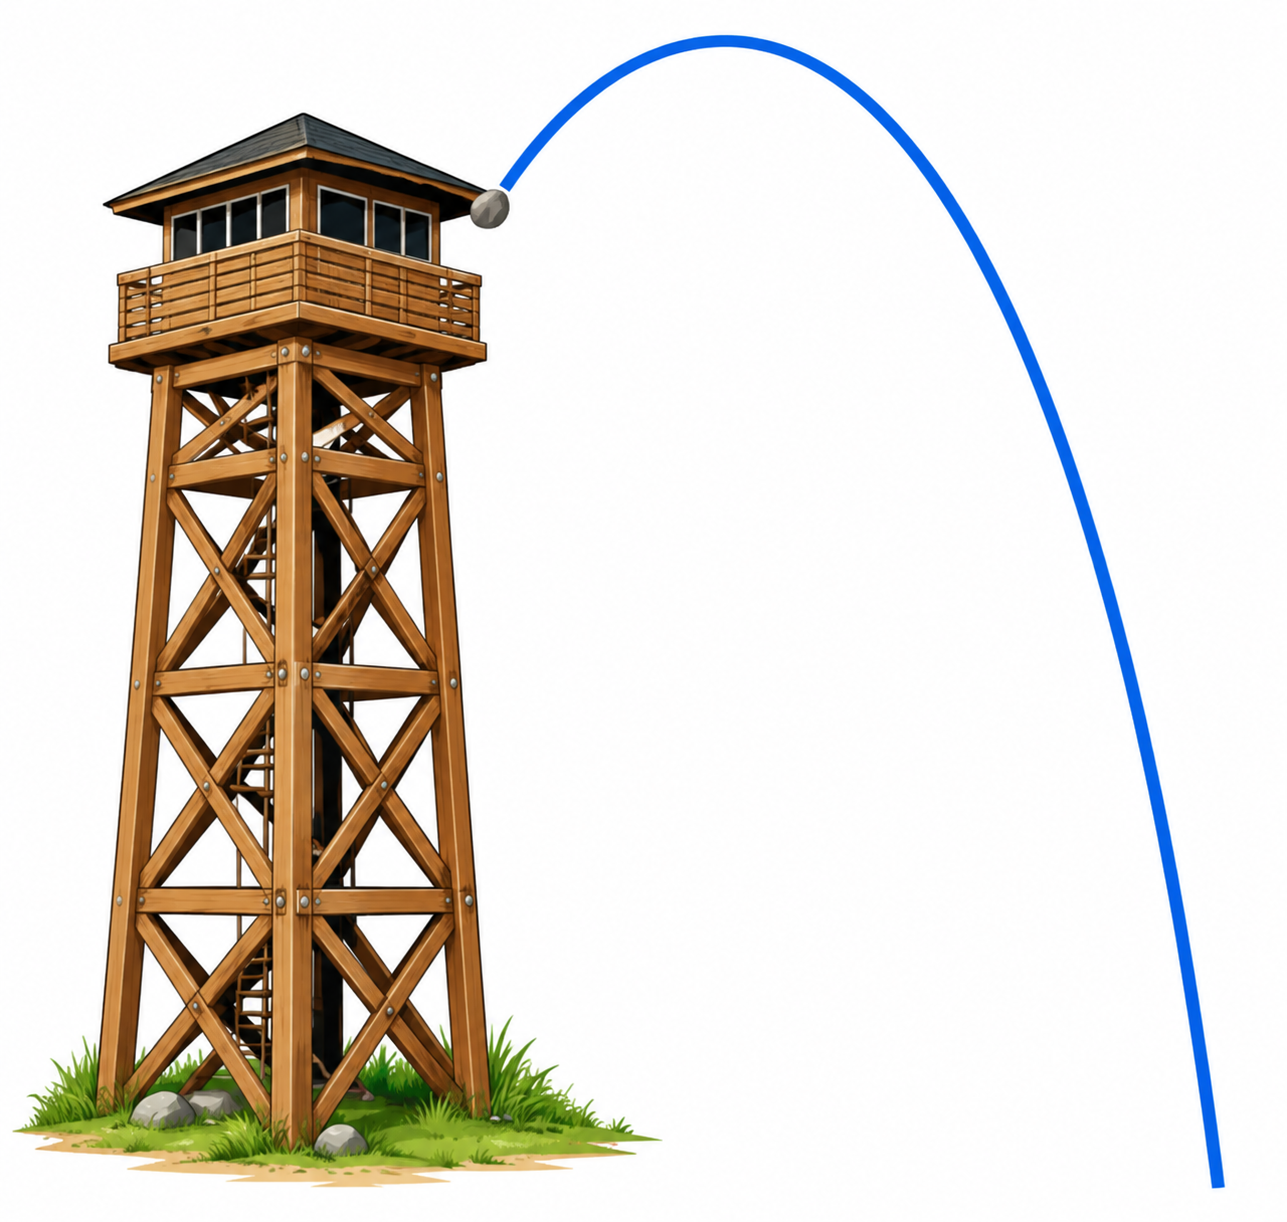
\includegraphics[width = 0.25 \textwidth]{media/Holzwachturm mit blauem Wurfparabel-Bogen.png}
    \end{center}
    Alice wirft einen Stein von einem Aussichtsturm.

    Die Flugphase des Steins kann durch die folgende Funktion
    beschrieben werden:
    \[
        h(t)=-5t^2+5t+30
    \]

    Dabei ist \(h(t)\) die Höhe des Steins über dem Boden
    (in Metern) und \(t\) bezeichnet die Zeit, die seit dem
    Abwurf verstrichen ist (in Sekunden).

    \begin{enumerate}
        \item Vervollständigen Sie die Wertetabelle:
              \begin{center}
                  \renewcommand{\arraystretch}{1.8}
                  \begin{tabular}{|c||*{7}{>{\centering\arraybackslash}p{1.5cm}|}}
                      \hline
                      \(t\)    & 0 & 0.5 & 1 & 1.5 & 2 & 2.5 & 3 \\ \hline
                      \(h(t)\) &   &     &   &     &   &     &   \\[8pt] \hline
                  \end{tabular}
              \end{center}
              %   \begin{center}
              %       \renewcommand{\arraystretch}{1.8}
              %       \begin{tabular}{|c||c|c|c|c|c|c|c|}
              %           \hline
              %           \(t\)    & 0 & 0.5 & 1 & 1.5 & 2 & 2.5 & 3 \\ \hline
              %           \(h(t)\) &   &     &   &     &   &     &   \\[8pt] \hline
              %       \end{tabular}
              %   \end{center}

        \item Zeichnen Sie den Graphen der Funktion \(h\) in das Koordinatensystem unten.

              \begin{center}
                  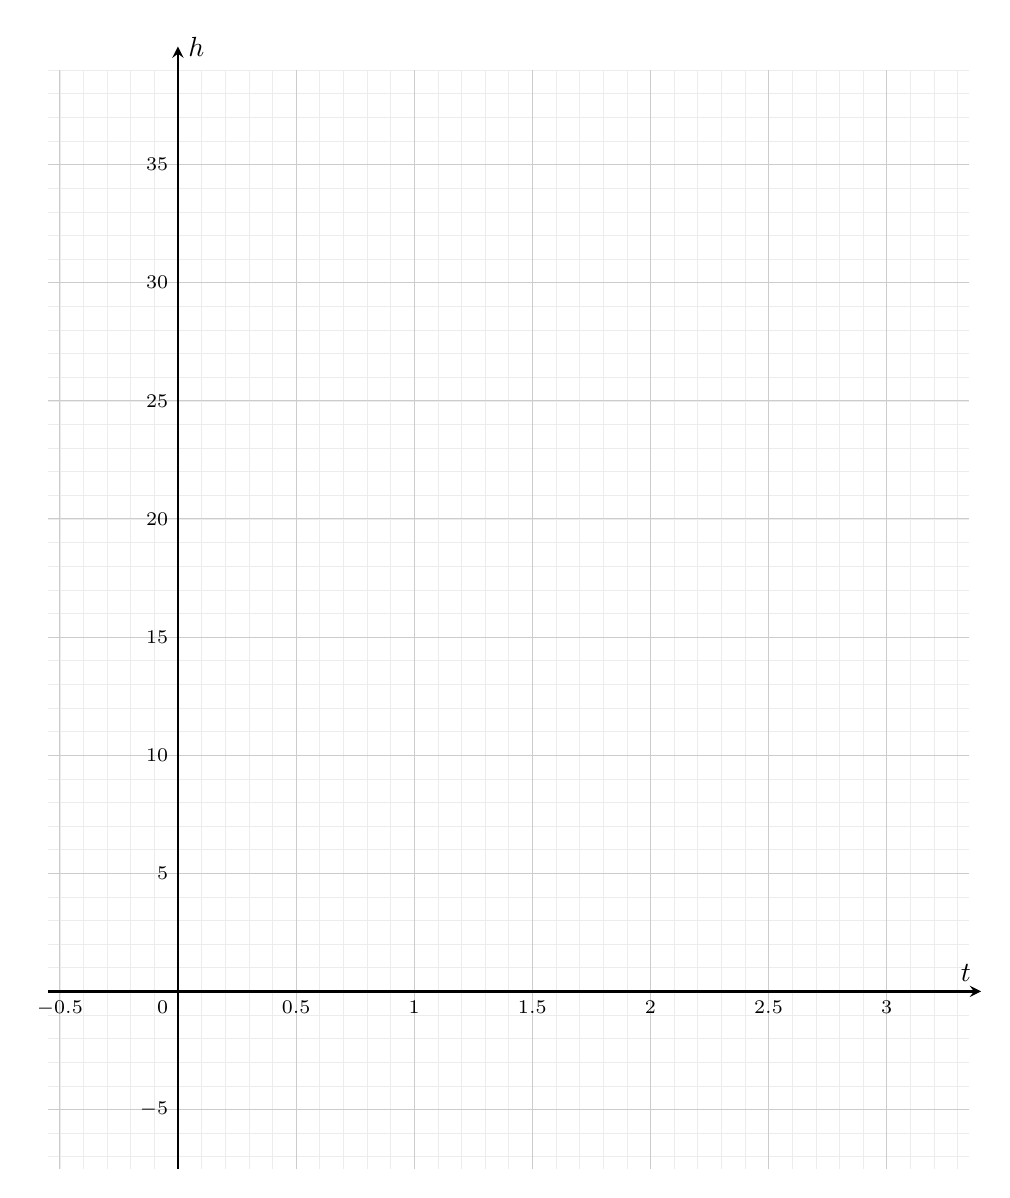
\begin{tikzpicture}[x=3cm, y=0.3cm, >=stealth]

                      % Feines Raster: 0.1 s und 1 m
                      \draw[xstep=0.1, ystep=1, gray!15, very thin]
                      (-0.55,-7.5) grid (3.35,39);

                      % Hauptlinien: 0.5 s und 5 m
                      \foreach \x in {-0.5,0,...,3}
                      \draw[gray!40, thin]
                      (\x,-7.5) -- (\x,39);

                      \foreach \y in {-5,0,...,35}
                      \draw[gray!40, thin]
                      (-0.55,\y) -- (3.35,\y);

                      % Achsen
                      \draw[->, thick]
                      (-0.55,0) -- (3.4,0)
                      node[above left] {\(t\)};

                      \draw[->, thick]
                      (0,-7.5) -- (0,40)
                      node[right] {\(h\)};

                      % Beschriftung der t-Achse
                      \foreach \x in {-0.5,0.5,1,1.5,2,2.5,3}
                      \node[below, font=\scriptsize]
                      at (\x,0) {\(\x\)};

                      % Ursprung
                      \node[below left, font=\scriptsize]
                      at (0,0) {\(0\)};

                      % Beschriftung der h-Achse
                      \foreach \y in {-5,5,10,15,20,25,30,35}
                      \node[left, font=\scriptsize]
                      at (0,\y) {\(\y\)};

                  \end{tikzpicture}
              \end{center}

        \item Auf welcher Höhe wurde der Stein abgeworfen?
              Welcher Punkt im Graphen liefert diese Information?

        \item Wie lange fliegt der Stein am Anfang noch nach oben?
              Wie lange dann nach unten? Wie erkennt man diese beiden
              Flugphasen am Graphen der Funktion?

        \item Wie lange dauert es, bis der Stein auf dem Boden
              landet? Welcher Punkt des Graphen liefert diese Information?

        \item \textbf{Challenge:}
              Welche Gleichung müsste man lösen, um die Frage 5.
              zu beantworten? Lösen Sie sie!
    \end{enumerate}
\end{LA}

\clearpage
Die Einstiegsaufgabe macht deutlich, dass Eigenschaften von Funktionsgraphen wichtige Informatio-
nen über die Funktion selbst liefern. Einige dieser Merkmale von Graphen spielen so häufig eine wichtige Rolle, dass sie in der Sprache der Mathematik eigene Namen erhalten haben.
\begin{definition}
    {Nullstellen}{NST}
    Sei \(f\colon \DD \to \WW\) eine Funktion. Ein Input \(x_0 \in \DD\)
    mit der Eigenschaft, dass
    \[
        f(x_0)=0
    \]
    ist, heisst \textbf{Nullstelle} der Funktion.

    Die Nullstellen sind diejenigen Stellen, an denen der Graph
    der Funktion die \(x\)-Achse schneidet.
\end{definition}

\begin{bsp}
    {Nullstellen einer quadratischen Funktion}{IntroNst}
    Die Nullstellen der Funktion \(h(t)=-5t^2+5t+30\) sind
    die Lösungen der Gleichung \(h(t)=0\):
    \[
        h(t)=0 \iff -5t^2+5t+30=0
    \]

    Da es sich nicht um eine lineare Gleichung handelt
    (wegen dem Quadrat), muss sie auf die Form
    \enquote{Produkt = 0} umgewandelt werden:
    \[
        -5t^2+5t+30=0
        \iff -5(t^2-t-6)=0
        \iff -5(t-3)(t+2)=0
    \]

    Die beiden Nullstellen der Funktion können nun
    herausgelesen werden:
    \[
        t_1=3,\qquad t_2=-2
    \]

    An diesen beiden Stellen schneidet der Graph der Funktion
    \(h\) die horizontale Achse:

    \begin{center}
        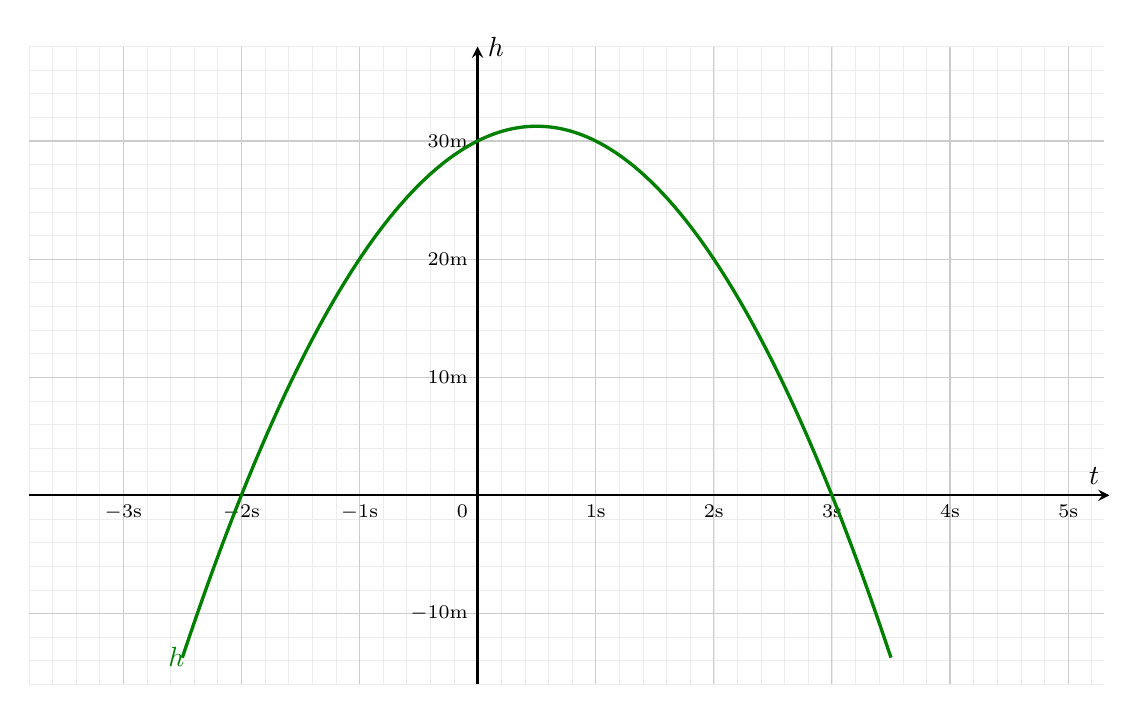
\begin{tikzpicture}[x=1.5cm,y=0.15cm,>=stealth]

            % Feines Raster
            \draw[xstep=0.2,ystep=2,gray!15,very thin]
            (-3.8,-16) grid (5.3,38);

            % Hauptlinien
            \foreach \x in {-3,...,5}
            \draw[gray!40,thin]
            (\x,-16) -- (\x,38);

            \foreach \y in {-10,0,10,20,30}
            \draw[gray!40,thin]
            (-3.8,\y) -- (5.3,\y);

            % Achsen
            \draw[->,thick]
            (-3.8,0) -- (5.35,0)
            node[above left] {\(t\)};

            \draw[->,thick]
            (0,-16) -- (0,38)
            node[right] {\(h\)};

            % Beschriftung der t-Achse
            \foreach \x in {-3,-2,-1,1,2,3,4,5}
            \node[below,font=\scriptsize]
            at (\x,0) {\(\x\mathrm{s}\)};

            \node[below left,font=\scriptsize]
            at (0,0) {\(0\)};

            % Beschriftung der h-Achse
            \foreach \y in {-10,10,20,30}
            \node[left,font=\scriptsize]
            at (0,\y) {\(\y\mathrm{m}\)};

            % Funktionsgraph
            \draw[green!50!black,very thick,
                domain=-2.5:3.5,samples=201,smooth]
            plot (\x,{-5*\x*\x+5*\x+30});

            \node[green!50!black,below left]
            at (-2.4,-12) {\(h\)};

        \end{tikzpicture}
    \end{center}


\end{bsp}
Auch der Schnittpunkt mit der vertikalen Achse hat einen eigenen Namen:
\begin{definition}
    {\(y\)-Achsenabchnitt}{}
    Sei \(f\colon \DD \to \WW\) eine Funktion. Die \(y\)-Koordinate
    \(y_0 \in \WW\) des Schnittpunktes des Graphen mit der
    \(y\)-Achse heisst \textbf{\(y\)-Achsenabschnitt}.

    Der \(y\)-Achsenabschnitt ist der Funktionswert an der
    Stelle Null:
    \[
        y_0=f(0).
    \]
\end{definition}
Die Funktion aus \Cref{bsp:IntroNst} hat den
\(y\)-Achsenabschnitt \(y_0=h(0)=30\).

An dieser Stelle sei auch bemerkt, dass nicht jede Funktion
Nullstellen und/oder einen \(y\)-Achsenabschnitt besitzt.
So hat die Funktion
\[
    g(x)=\sqrt{x-1}+2
\]
weder das eine noch das andere (siehe Bild).

\begin{center}
    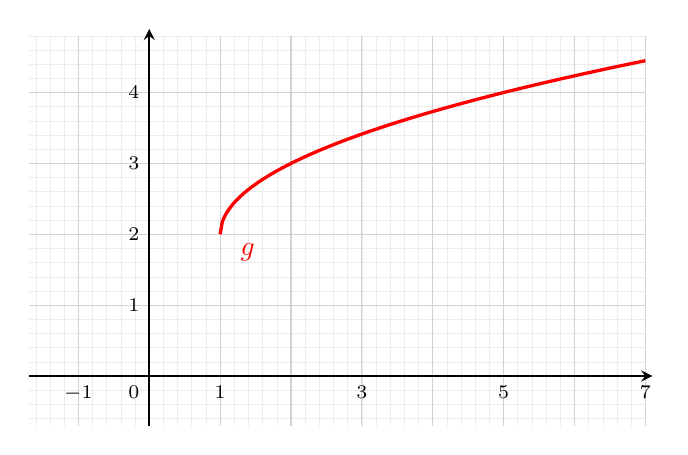
\begin{tikzpicture}[x=0.9cm,y=0.9cm,>=stealth]

        % Feines Raster
        \draw[xstep=0.2,ystep=0.2,gray!15,very thin]
        (-1.7,-0.7) grid (7,4.8);

        % Hauptlinien
        \foreach \x in {-1,...,7}
        \draw[gray!35,thin]
        (\x,-0.7) -- (\x,4.8);

        \foreach \y in {0,...,4}
        \draw[gray!35,thin]
        (-1.7,\y) -- (7,\y);

        % Achsen
        \draw[->,thick] (-1.7,0) -- (7.1,0);
        \draw[->,thick] (0,-0.7) -- (0,4.9);

        % Achsenbeschriftung
        \foreach \x in {-1,1,...,7}
        \node[below,font=\scriptsize]
        at (\x,0) {\(\x\)};

        \node[below left,font=\scriptsize]
        at (0,0) {\(0\)};

        \foreach \y in {1,...,4}
        \node[left,font=\scriptsize]
        at (0,\y) {\(\y\)};

        % Funktionsgraph
        \draw[red,very thick,domain=1:7,samples=201]
        plot (\x,{sqrt(\x-1)+2});

        \node[red,below right] at (1.15,2) {\(g\)};

    \end{tikzpicture}
\end{center}

Oft ist es wichtig zu wissen, ob die Funktionswerte in einem bestimmten Teilbereich der Definitions-
menge ansteigen oder fallen.

\begin{definition}
    {Monotonie}{}
    Eine Funktion \(f\colon \DD \to \WW\) heisst
    \textbf{monoton wachsend}, falls für alle
    \(x_1 < x_2\) mit \(x_1,x_2 \in \DD\) gilt, dass
    \(f(x_1) \leq f(x_2)\) ist.

    Sie heisst \textbf{streng monoton wachsend}, falls für alle
    \(x_1 < x_2\) mit \(x_1,x_2 \in \DD\) gilt, dass
    \(f(x_1) < f(x_2)\) ist.

    \medskip

    Analog werden auch die Begriffe \textbf{monoton fallend}
    und \textbf{streng monoton fallend} definiert.
\end{definition}

\begin{bsp}
    {Monotonie bei einer quadratischen Funktion}{}
    Die Funktion aus der Einstiegsaufgabe ist streng monoton wachsend
    im Intervall \(]-\infty,\frac{1}{2}]\) und streng monoton fallend
    im Intervall \([\frac{1}{2},\infty[\).

    \begin{center}
        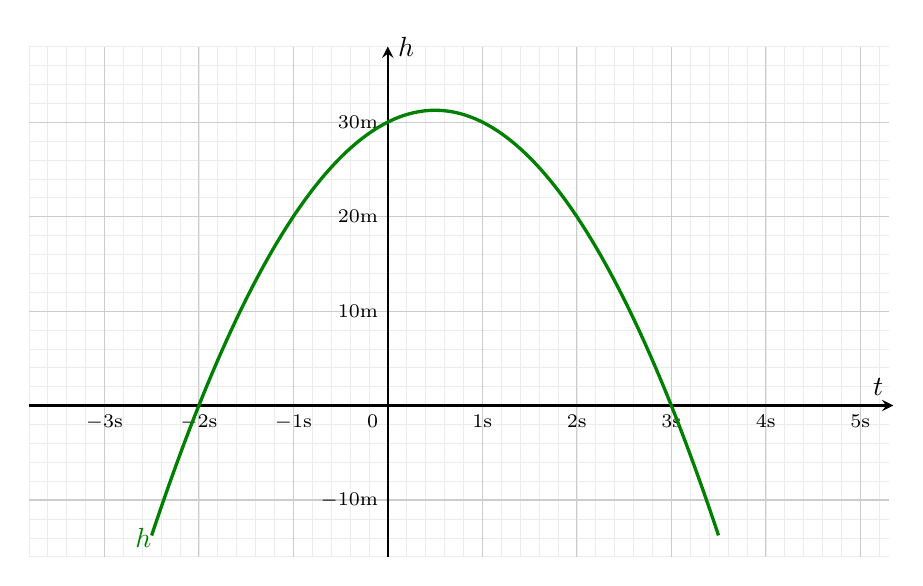
\begin{tikzpicture}[x=1.2cm,y=0.12cm,>=stealth]

            % Feines Raster
            \draw[xstep=0.2,ystep=2,gray!15,very thin]
            (-3.8,-16) grid (5.3,38);

            % Hauptlinien
            \foreach \x in {-3,...,5}
            \draw[gray!40,thin]
            (\x,-16) -- (\x,38);

            \foreach \y in {-10,0,10,20,30}
            \draw[gray!40,thin]
            (-3.8,\y) -- (5.3,\y);

            % Achsen
            \draw[->,thick]
            (-3.8,0) -- (5.35,0)
            node[above left] {\(t\)};

            \draw[->,thick]
            (0,-16) -- (0,38)
            node[right] {\(h\)};

            % Beschriftung der t-Achse
            \foreach \x in {-3,-2,-1,1,2,3,4,5}
            \node[below,font=\scriptsize]
            at (\x,0) {\(\x\mathrm{s}\)};

            \node[below left,font=\scriptsize]
            at (0,0) {\(0\)};

            % Beschriftung der h-Achse
            \foreach \y in {-10,10,20,30}
            \node[left,font=\scriptsize]
            at (0,\y) {\(\y\mathrm{m}\)};

            % Funktionsgraph
            \draw[green!50!black,very thick,
                domain=-2.5:3.5,samples=201,smooth]
            plot (\x,{-5*\x*\x+5*\x+30});

            \node[green!50!black,below left]
            at (-2.4,-12) {\(h\)};

        \end{tikzpicture}
    \end{center}
\end{bsp}

\begin{bsp}
    {Monotonie bei der Abrundungsfunktion}{}
    Die Abrundungsfunktion wird mit \(\operatorname{floor}(x)\) oder
    \(\lfloor x \rfloor\) bezeichnet. Sie ordnet jeder reellen Zahl \(x\)
    die grösste ganze Zahl \(n \leq x\) zu. Zum Beispiel
    \(\lfloor \pi \rfloor = 3\) oder
    \(\left\lfloor -\frac{3}{4} \right\rfloor = -1\)
    oder \(\lfloor 5 \rfloor = 5\).

    Der Graph der Abrundungsfunktion sieht wie folgt aus:

    \begin{center}
        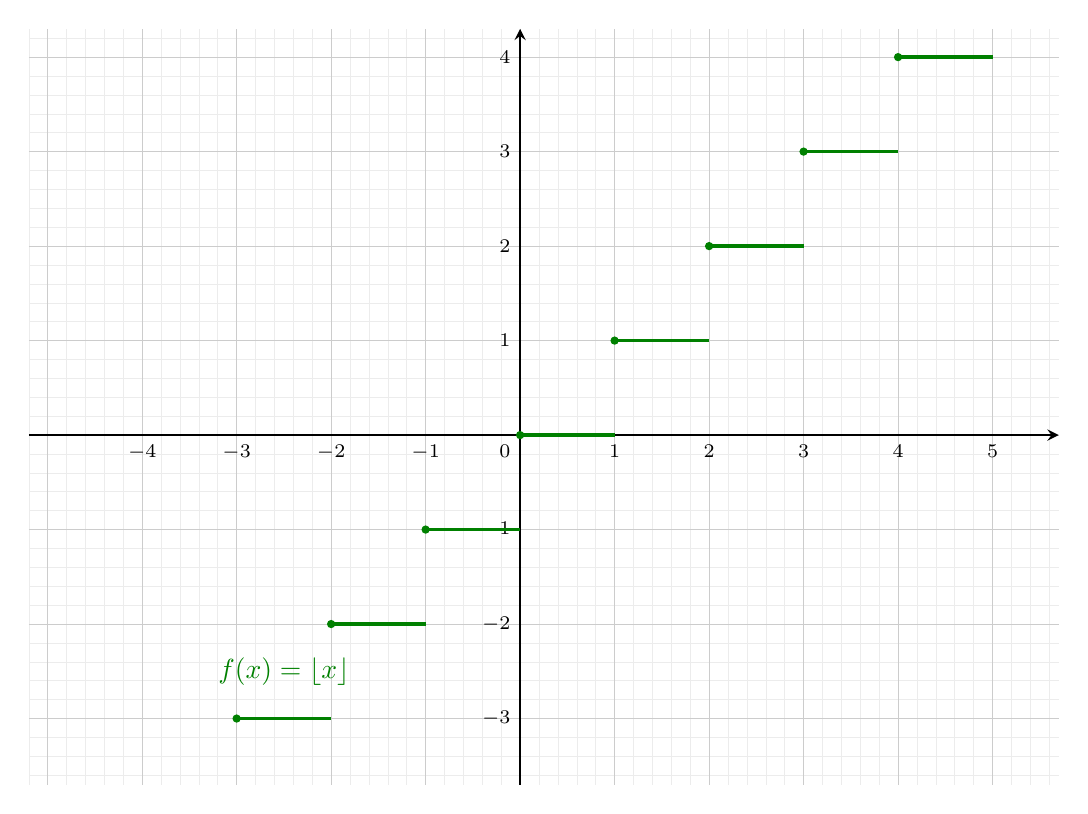
\begin{tikzpicture}[x=1.2cm,y=1.2cm,>=stealth]

            % Feines Raster
            \draw[xstep=0.2,ystep=0.2,gray!15,very thin]
            (-5.2,-3.7) grid (5.7,4.3);

            % Hauptlinien
            \foreach \x in {-5,...,5}
            \draw[gray!40,thin]
            (\x,-3.7) -- (\x,4.3);

            \foreach \y in {-3,...,4}
            \draw[gray!40,thin]
            (-5.2,\y) -- (5.7,\y);

            % Achsen
            \draw[->,thick] (-5.2,0) -- (5.7,0);
            \draw[->,thick] (0,-3.7) -- (0,4.3);

            % Achsenbeschriftung
            \foreach \x in {-4,-3,-2,-1,1,2,3,4,5}
            \node[below,font=\scriptsize] at (\x,0) {\(\x\)};

            \node[below left,font=\scriptsize] at (0,0) {\(0\)};

            \foreach \y in {-3,-2,-1,1,2,3,4}
            \node[left,font=\scriptsize] at (0,\y) {\(\y\)};

            % Abrundungsfunktion
            \foreach \n in {-3,-2,-1,0,1,2,3,4} {
                    \draw[green!50!black,very thick]
                    (\n,\n) -- ({\n+1},\n);

                    \fill[green!50!black] (\n,\n) circle (1.5pt);

                    % \draw[green!50!black,fill=white]
                    % ({\n+1},\n) circle (1.5pt);
                }

            % Funktionsbezeichnung
            \node[green!50!black] at (-2.5,-2.5)
            {\(f(x)=\lfloor x\rfloor\)};

        \end{tikzpicture}
    \end{center}

    Die Abrundungsfunktion ist \textbf{monoton wachsend},
    aber \textbf{nicht streng monoton wachsend}.
\end{bsp}























\clearpage
\subsection{Gerade und ungerade Funktionen}
\begin{LA}
    {Einstiegsaufgabe}{}
    Ziel der Aufgabe ist die Untersuchung von Funktionen mit Graphen,
    die punktsymmetrisch zum Ursprung oder achsensymmetrisch zur
    \(y\)-Achse verlaufen.

    \begin{enumerate}
        \item Betrachten Sie den Punkt \(P=(1, -3)\) im Koordinatensystem:

              \begin{center}
                  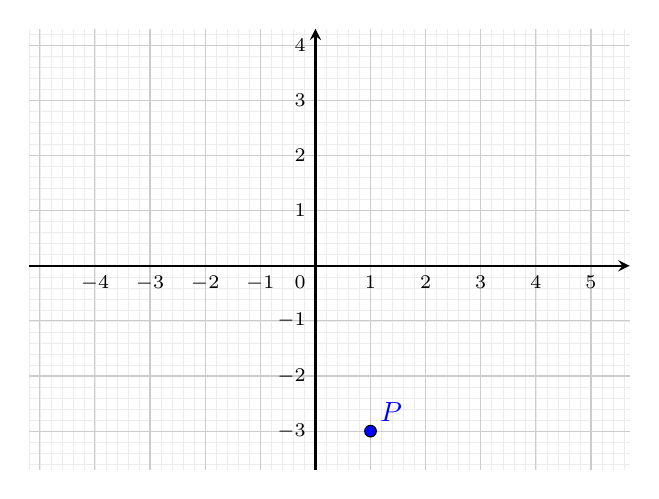
\begin{tikzpicture}[x=1cm,y=1cm,>=stealth, scale = 0.7]

                      % Feines Raster
                      \draw[xstep=0.2,ystep=0.2,gray!15,very thin]
                      (-5.2,-3.7) grid (5.7,4.3);

                      % Hauptlinien
                      \foreach \x in {-5,...,5}
                      \draw[gray!40,thin]
                      (\x,-3.7) -- (\x,4.3);

                      \foreach \y in {-3,...,4}
                      \draw[gray!40,thin]
                      (-5.2,\y) -- (5.7,\y);

                      % Achsen
                      \draw[->,thick] (-5.2,0) -- (5.7,0);
                      \draw[->,thick] (0,-3.7) -- (0,4.3);

                      % Beschriftung der x-Achse
                      \foreach \x in {-4,-3,-2,-1,1,2,3,4,5}
                      \node[below,font=\scriptsize]
                      at (\x,0) {\(\x\)};

                      \node[below left,font=\scriptsize]
                      at (0,0) {\(0\)};

                      % Beschriftung der y-Achse
                      \foreach \y in {-3,-2,-1,1,2,3,4}
                      \node[left,font=\scriptsize]
                      at (0,\y) {\(\y\)};

                      % Punkt P
                      \filldraw[blue,draw=black]
                      (1,-3) circle (3pt);

                      \node[blue,above right] at (1,-3) {\(P\)};

                  \end{tikzpicture}
              \end{center}

              Wohin kommt der Punkt \(P\) zu liegen nach einer Punktspiegelung
              mit Zentrum im Ursprung \(O=(0, 0)\)?
              Geben Sie die Koordinaten des Bildpunktes \(P'\) an:

        \item Gegeben ist nun die Funktion
              \[
                  f(x)=x(x-2)(x+2).
              \]

              \begin{enumerate}
                  \item Weisen Sie rechnerisch nach, dass der Punkt \(P\)
                        aus Aufgabe 1. auf dem Graphen von \(f\) liegt.

                  \item Liegt auch der Punkt \(P'\) auf dem Graphen von \(f\)?

                  \item Berechnen Sie die \(y\)-Koordinate von \(Q(3, ?)\),
                        sodass der Punkt auf dem Graphen von \(f\) liegt.
                        Liegt sein Spiegelpunkt \(Q'\) auch auf dem Graphen von \(f\)?

                  \item Wieso reichen die Erkenntnisse aus den Teilaufgaben
                        (a)--(c) nicht als Beweis, dass der Graph von \(f\)
                        punktsymmetrisch zum Ursprung verläuft?

                  \item Was müsste man prüfen, um Gewissheit über die
                        Punktsymmetrie des Graphen zu erlangen?
              \end{enumerate}

        \item \textbf{Challenge:} Betrachten Sie zum Schluss die Funktion
              \[
                  g(x)=\frac{1}{x^2+1}.
              \]
              Alice behauptet, der Graph der Funktion \(g\)
              verlaufe achsensymmetrisch bezüglich der \(y\)-Achse.
              Stimmt ihre Behauptung?

    \end{enumerate}
\end{LA}

\clearpage

Die Funktion \(f(x)=x(x-2)(x+2)\) aus der Einstiegsaufgabe
hat den Graphen unten.

\begin{center}
    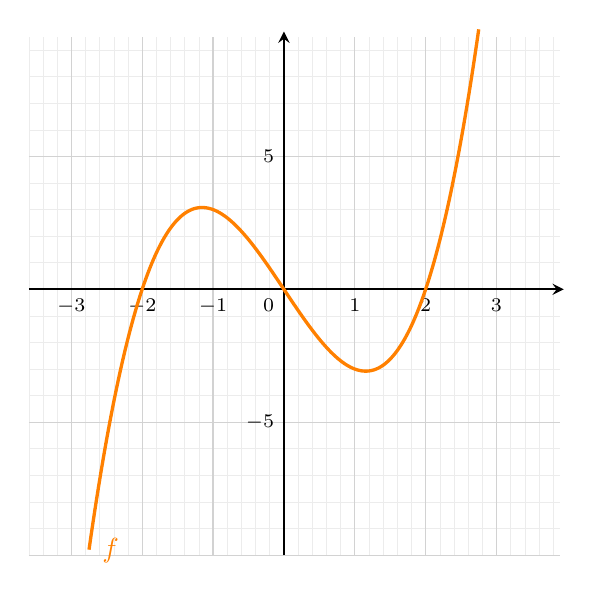
\begin{tikzpicture}[x=1.2cm,y=0.45cm,>=stealth, scale = 0.75]

        % Feines Raster
        \draw[xstep=0.2,ystep=1,gray!15,very thin]
        (-3.6,-10) grid (3.9,9.5);

        % Hauptlinien
        \foreach \x in {-3,...,3}
        \draw[gray!35,thin]
        (\x,-10) -- (\x,9.5);

        \foreach \y in {-10,-5,0,5}
        \draw[gray!35,thin]
        (-3.6,\y) -- (3.9,\y);

        % Achsen
        \draw[->,thick] (-3.6,0) -- (3.95,0);
        \draw[->,thick] (0,-10) -- (0,9.7);

        % Achsenbeschriftung
        \foreach \x in {-3,-2,-1,1,2,3}
        \node[below,font=\scriptsize]
        at (\x,0) {\(\x\)};

        \node[below left,font=\scriptsize]
        at (0,0) {\(0\)};

        \foreach \y in {-5,5}
        \node[left,font=\scriptsize]
        at (0,\y) {\(\y\)};

        % Funktionsgraph
        \draw[orange,very thick,domain=-2.75:2.75,
            samples=201,smooth]
        plot (\x,{\x*(\x-2)*(\x+2)});

        \node[orange,below right]
        at (-2.7,-9) {\(f\)};

    \end{tikzpicture}
\end{center}

Der Graph scheint punktsymmetrisch zum Ursprung zu verlaufen.
Wie kann man sich dessen aber sicher sein?
Das hiesse doch, dass beispielsweise die Funktionswerte
an den Stellen \(1\) und \(-1\) sich nur um das Vorzeichen
unterscheiden. Das stimmt offensichtlich, denn:
\begin{align*}
    f(1)  & = 1\cdot(1-2)\cdot(1+2)=-3,    \\
    f(-1) & = (-1)\cdot(-1-2)\cdot(-1+2)=3
\end{align*}

Die beiden Graphenpunkte \((-1, 3)\) und \((1, -3)\) liegen
demnach punktsymmetrisch zum Ursprung. Damit der ganze Graph
punktsymmetrisch zum Ursprung verläuft, müssen sich
\textbf{für jeden beliebigen Input} \(u\in\DD\)
die Funktionswerte an den Stellen \(u\) und
\(-u\) nur um das Vorzeichen unterscheiden:
\begin{align*}
    f(u)
     & = u\cdot(u-2)\cdot(u+2)
    = u^3-4u,                       \\
    f(-u)
     & = (-u)\cdot(-u-2)\cdot(-u+2)
    = -u^3+4u
\end{align*}

Also: \(f(-u)=-f(u)\).

\begin{definition}
    {Ungerade Funktion}{}
    Falls für eine Funktion \(f\colon \DD \to \WW\) gilt, dass
    \[
        f(-u)=-f(u)
        \qquad \text{für alle } u\in\DD,
    \]
    so verläuft der Graph der Funktion punktsymmetrisch zum Ursprung.

    Eine Funktion mit dieser Eigenschaft nennt man \textbf{ungerade}.
\end{definition}
Analog gibt es Funktionen deren Graphen achsensymmetrisch zur \(y\)-Achse verlaufen:
\begin{definition}
    {Gerade Funktion}{}
    Falls für eine Funktion \(f\colon \DD \to \WW\) gilt, dass
    \[
        f(-u)=f(u)
        \qquad \text{für alle } u\in\DD,
    \]
    so verläuft der Graph der Funktion achsensymmetrisch zur \(y\)-Achse.

    Eine Funktion mit dieser Eigenschaft nennt man \textbf{gerade}.
\end{definition}
\begin{bsp}
    {Gerade Funktion}{geradeFunktion}
    Die Funktion \(g(x)=\frac{1}{x^2+1}\) ist gerade, denn
    \[
        g(u)=\frac{1}{u^2+1},
        \qquad
        g(-u)=\frac{1}{(-u)^2+1}
        =\frac{1}{u^2+1}.
    \]

    Also gilt für alle \(u\in\DD\):
    \(g(-u)=g(u)\).

    \begin{center}
        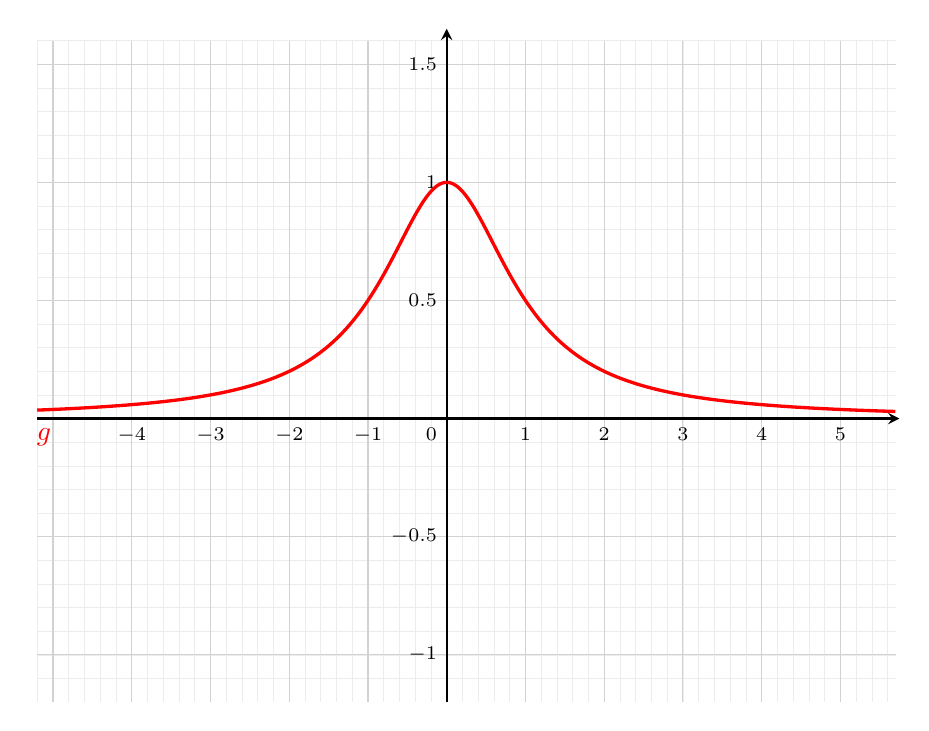
\begin{tikzpicture}[x=1cm,y=3cm,>=stealth]

            % Feines Raster
            \draw[xstep=0.2,ystep=0.1,gray!15,very thin]
            (-5.2,-1.2) grid (5.7,1.6);

            % Hauptlinien
            \foreach \x in {-5,...,5}
            \draw[gray!35,thin]
            (\x,-1.2) -- (\x,1.6);

            \foreach \y in {-1,-0.5,0,0.5,1,1.5}
            \draw[gray!35,thin]
            (-5.2,\y) -- (5.7,\y);

            % Achsen
            \draw[->,thick] (-5.2,0) -- (5.75,0);
            \draw[->,thick] (0,-1.2) -- (0,1.65);

            % Beschriftung der x-Achse
            \foreach \x in {-4,-3,-2,-1,1,2,3,4,5}
            \node[below,font=\scriptsize]
            at (\x,0) {\(\x\)};

            \node[below left,font=\scriptsize]
            at (0,0) {\(0\)};

            % Beschriftung der y-Achse
            \foreach \y in {-1,-0.5,0.5,1,1.5}
            \node[left,font=\scriptsize]
            at (0,\y) {\(\y\)};

            % Funktionsgraph
            \draw[red,very thick,domain=-5.2:5.7,
                samples=201,smooth]
            plot (\x,{1/(\x*\x+1)});

            \node[red,below left]
            at (-4.9,0) {\(g\)};

        \end{tikzpicture}
    \end{center}
\end{bsp}
Neben den in diesem Kapitel besprochenen Eigenschaften von Graphen gibt es viele andere, die zum Teil zu einem späteren Zeitpunkt behandelt werden: Periodizität, Krümmungsverhalten, Wendepunkte, lokale Extrema, asymptotisches Verhalten und viele mehr.

\begin{ueb}
    {}{}


    \begin{enumerate}
        \item \(f(x)=\frac{3}{10}x-6\)
              \begin{enumerate}
                  \item Bestimmen Sie die Nullstelle(n).
                  \item Bestimmen Sie den \(y\)-Achsenabschnitt.
                  \item Ist die Funktion monoton wachsend oder fallend?
              \end{enumerate}

        \item \(g(x)=-x^2+9\)
              \begin{enumerate}
                  \item Bestimmen Sie die Nullstelle(n).
                  \item Bestimmen Sie den \(y\)-Achsenabschnitt.
                  \item Beweisen Sie, dass die Funktion gerade ist.
              \end{enumerate}

        \item \(h(x)=x^3-x\)
              \begin{enumerate}
                  \item Bestimmen Sie die Nullstelle(n).
                  \item Bestimmen Sie den \(y\)-Achsenabschnitt.
                  \item Beweisen Sie, dass die Funktion ungerade ist.
              \end{enumerate}

        \item \(i(x)=2\sqrt{5x+16}\)
              \begin{enumerate}
                  \item Bestimmen Sie die Nullstelle(n).
                  \item Bestimmen Sie den \(y\)-Achsenabschnitt.
                  \item Ist die Funktion monoton wachsend oder fallend?
              \end{enumerate}

        \item Geben Sie eine möglichst einfache Funktion an mit
              \begin{enumerate}
                  \item \(y\)-Achsenabschnitt \(y_0=5\).
                  \item \(y\)-Achsenabschnitt \(y_0=2\) und Nullstelle \(x_0=4\).
                  \item den Nullstellen \(x_1=-2\), \(x_2=2\).
                  \item ohne Nullstellen.
                  \item ohne \(y\)-Achsenabschnitt.
              \end{enumerate}

        \item Geben Sie für jede der folgenden Funktionen den
              \(y\)-Achsenabschnitt und alle Nullstellen an.
              Entscheiden Sie ausserdem, ob es sich um gerade oder
              ungerade Funktionen handelt, und geben Sie Teilmengen
              des Definitionsbereichs an, auf welchen die Funktion
              (streng) monoton ist.
              \begin{enumerate}
                  \item Betragsfunktion \(y=|x|\).
                  \item Vorzeichenfunktion \(y=\operatorname{sgn}(x)\).
                  \item Kehrwertfunktion \(y=\frac{1}{x}\).
              \end{enumerate}

              % \item Bestimmen Sie die Nullstellen der Funktion \(g\).

              %       \begin{enumerate}
              %           \item \(g(x)=(x+1)(x^2-5)\)
              %           \item \(g(x)=\dfrac{x^3-x}{x^3+2x+3}\)
              %           \item \(g(z)=z+|z|\)
              %           \item \(g(x)=\dfrac{5}{x}\)
              %       \end{enumerate}

        \item Es gibt eine Funktion, die gerade, ungerade,
              monoton wachsend und monoton fallend ist. Welche?
    \end{enumerate}
\end{ueb}

\clearpage
\textbf{Lösungen:}
\begin{enumerate}
    \item Nullstelle \(x=20\), \(y\)-Achsenabschnitt \(y_0=-6\),
          streng monoton wachsend.

    \item Nullstellen \(x_1=-3\), \(x_2=3\),
          \(y\)-Achsenabschnitt \(y_0=9\).
          \[
              g(-u)
              =-(-u)^2+9
              =-u^2+9
              =g(u)
              \quad\Rightarrow\quad \text{gerade}.
          \]

    \item Nullstellen \(x_1=-1\), \(x_2=0\), \(x_3=1\),
          \(y\)-Achsenabschnitt \(y_0=0\).
          \[
              h(-u)
              =(-u)^3-(-u)
              =-u^3+u
              =-(u^3-u)
              =-h(u)
              \quad\Rightarrow\quad \text{ungerade}.
          \]

    \item \(i(x)=2\sqrt{5x+16}\):
          Nullstelle \(x_0=-\frac{16}{5}\),
          \(y\)-Achsenabschnitt \(y_0=8\),
          streng monoton wachsend.

    \item Geben Sie eine möglichst einfache Funktion an mit
          (mögliche Antworten):
          \begin{enumerate}
              \item \(y=5\)
              \item \(y=-\frac12 x+2\)
              \item \(y=x^2-4\)
              \item \(y=5\)
              \item \(y=\frac1x\)
          \end{enumerate}

    \item Geben Sie für jede der folgenden Funktionen den
          \(y\)-Achsenabschnitt und alle Nullstellen an.
          Entscheiden Sie ausserdem, ob es sich um gerade oder
          ungerade Funktionen handelt, und geben Sie Teilmengen
          des Definitionsbereichs an, auf welchen die Funktion
          (streng) monoton ist.

          \begin{enumerate}
              \item \textbf{Betragsfunktion:}

                    Nullstelle \(x_0=0\), \(y\)-Achsenabschnitt \(y_0=0\),
                    gerade, streng monoton fallend auf
                    \(\mathbb R_0^-\), streng monoton wachsend auf
                    \(\mathbb R_0^+\).

              \item \textbf{Vorzeichenfunktion:}

                    Nullstelle \(x_0=0\), \(y\)-Achsenabschnitt \(y_0=0\),
                    ungerade, monoton wachsend auf \(\mathbb R\).

              \item \textbf{Kehrwertfunktion:}

                    Keine Nullstellen, kein \(y\)-Achsenabschnitt,
                    ungerade, streng monoton fallend auf
                    \(]-\infty,0[\) und auf \(]0,\infty[\).

                    Der Definitionsbereich ist
                    \[
                        \DD=\mathbb R\setminus\{0\}.
                    \]
          \end{enumerate}

    \item \(y=0\)
\end{enumerate}